\documentclass[10pt]{article}

%---------------------------------------------------------------------
\usepackage[a4paper, headsep=-4in,bindingoffset=0in,%
left=2.5cm,right=2.5cm,top=2.5cm,bottom=2.5cm,%
footskip=.25in]{geometry}
\newcommand{\textBF}[1]{%
    \pdfliteral direct {2 Tr 0.3 w} %the second factor is the boldness
     #1%
    \pdfliteral direct {0 Tr 0 w}%
}
\usepackage{multirow}
\usepackage{soul}

\usepackage{xr}
\externaldocument{main}
\def\Plus{\texttt{+}}
%\usepackage[english]{babel}   
\usepackage[utf8]{inputenc}  
\usepackage[font=scriptsize]{caption}
\usepackage{tabularx}
%\DeclareCaptionFont{6pt}{\fontsize{6pt}{6pt}\selectfont}
\captionsetup[figure]{font={stretch=1}}  
%\usepackage{sectsty}
\usepackage{subcaption}
\usepackage{wrapfig}
\usepackage{layout}
\usepackage{graphicx}
\usepackage{verbatim}
\usepackage{listings}
\usepackage{mathptmx}

\usepackage{booktabs}
\usepackage{etoolbox}

\newcommand{\beginsupplement}{%
\setcounter{table}{0}
\renewcommand{\thetable}{S\arabic{table}}%
\setcounter{figure}{0}
\renewcommand{\thefigure}{S\arabic{figure}}%
}

\usepackage{lmodern}
\usepackage[T1]{fontenc}
\usepackage[backend=biber,style=apa,sorting=none]{biblatex}
\addbibresource{paperpile.bib}
%\pagenumbering{gobble}
\pagenumbering{arabic}

\graphicspath{{figs/}}
\setlength{\topmargin}{-10pt}
%\renewcommand{\baselinestretch}{1.5}

\usepackage{indentfirst}
\setlength{\parindent}{1cm}
\usepackage[table]{xcolor}
\setlength{\headsep}{1pt}

\begin{document} 

\begin{center}
{\large \section*{Systematic comparison of imaging biomarkers of chronic stroke motor outcome in the ENIGMA Stroke Recovery Working Group dataset}}
\end{center}

\begin{center}
Emily Olafson$^1$, Keith Jamison$^1$, Amy Kuceyeski$^1$
\end{center}

    1. \textmd{Department of Radiology, Weill Cornell Medical College, New York City, New York, USA, 10021} 

%---------------------------------------------------------------------

\section{Abstract}
Ischemic stroke is a major cause of physical impairment, and up to a third of stroke survivors have poor motor outcomes five years after the event. However, the ability to predict long-term deficits from acute clinical information remains a challenge. Incorporating information about lesion location can improve prediction models, but it is unclear how to optimally use volumetric lesion data to predict chronic motor outcomes. Several lesion biomarkers have been related to stroke motor outcome, but it is unclear whether they can accurately predict chronic impairments across a range of lesion topographies. Models that incorporate damage to additional sensorimotor regions beyond the primary motor cortex have been shown to explain more variance in post-stroke outcome than models that only incorporate primary motor cortex CST damage. These models typically incorporate damage to premotor, supplementary motor, pre-supplementary motor, and somatosensory cortices. Few studies have assessed the performance of these models with cross-validation. This paper presents a comparison of the predictive accuracy of several imaging biomarkers of post-stroke motor impairment using the ENIGMA dataset, a multi-site stroke lesion database. The models are compared using out-of-sample performance, and the results show that data-driven features outperform theory-driven features. The data-driven features also outperform models trained on chronic subjects when applied to acute subjects. These results highlight the potential of data-driven feature selection in identifying lesion-deficit associations beyond current theory-driven biomarkers.

\section{Introduction}
Ischemic stroke is a leading cause of physical impairment worldwide. Up to one-third of stroke survivors have poor motor outcomes five years after stroke, but the ability to predict long-term deficits from acute clinical information is still a major challenge.

The location of the stroke in the brain explains some of the variance in long-term outcomes, and models of stroke outcome are improved by incorporating information about lesion location. Lesion segmentations, once requiring  delineation by experts, can now be performed with automated methods requiring minimal manual editing (\cite{Pustina2016-qu}). However, it is currently unclear how to optimally relate lesion data to chronic motor outcomes (\cite{Sperber2020-kp, Kasties2021-rm}), and to what extent lesion data can predict deficits in new patients.

Several biomarkers of stroke motor outcomes have been derived from lesion data. The most widely-employed is the corticospinal tract (CST) lesion load, or the proportion of voxels in the ipsilesional corticospinal tract (typically originating from primary motor cortex) that intersect with the lesion (\cite{Zhu2010-qh, Feng2015-du, Findlater2019-je}). This biomarker has been related to motor deficits in the acute phase of stroke, but it is unclear whether this biomarker can accurately predict chronic impairments across a wide range of lesion topographies (for review, see \cite{Kim2017-xe}). Models that incorporate information about how the lesion damages secondary sensorimotor regions, i.e. regions beyond the primary motor cortex that are still related to motor behavior, explain more variance in post-stroke outcome than models that incorporate information about primary motor cortex CST damage alone (\cite{Ito2022-em, Sperber2021-lw, Rondina2016-ds, Rondina2017-ij, Schulz2012-yy}). For instance, \cite{Ito2022-em} have shown that models that use lesion load of sensorimotor tracts, specifically tracts originating from the ventral premotor cortex, better predict stroke motor severity compared to models that only use M1-CST-LL. These more complex models tend to incorporate damage to premotor, supplementary motor, pre-supplementary motor, and somatosensory cortices (\cite{Ito2022-em,Schulz2012-yy, Sperber2021-lw, Rondina2016-ds, Rondina2017-ij}).

Variables that are significantly associated with outcomes (typically derived from an inference-based, hypothesis-testing framework), may not be the optimal set of variables to use in predictive models (\cite{Bzdok2020-py}). Indeed, the optimal set of features extracted from lesion data may not be directly related to hemiparesis per se (\cite{Sperber2021-lw}). Because of the hierarchical and non-random distribution of lesion topography (\cite{Mah2014-cb,Wang2019-dz}), damage to areas outside of the motor system may meaningfully predict chronic motor impairment (\cite{Sperber2021-lw}). Machine learning models that incorporate features in a data-driven way may be able to discover lesion-deficit associations beyond the current suite of theory-based biomarkers like those in the motor system (\cite{Kasties2021-rm, Calesella2021-kp}). We estimated structural disconnection of all gray matter regions in the brain using the Network Modification tool (\cite{Kuceyeski2013-nk}) and used data-driven feature selection to identify regions that were relevant for predicting chronic motor outcomes. 

The ultimate application of stroke lesion biomarkers is to predict future deficit scores for patients in whom only imaging, or other limited clinical data, is available. Doing so will require machine learning models whose parameters have been optimized through prior training on stroke datasets. Most lesion-based biomarkers have been related to motor deficits within a clinical sample, but few studies have assessed whether those models perform well on new data. 

The goal of this paper is to compare the predictive performance of several imaging biomarkers of chronic post-stroke motor deficits using a large, heterogeneous stroke population. We compare the benchmark imaging biomarker, M1 corticospinal tract lesion load (\cite{Boyd2017-gs}), with  high-dimensional models that model motor deficits as a function of of structural damage to 1) the wider sensorimotor system and 2) the entire brain. We evaluate the performance of feature selection 


\cite{Park2016-te} Quantification of structural damage can add to models explaining motor outcome after stroke, but assessment of corticospinal tract damage alone is unlikely to be sufficient when considering patients with stroke with a wide range of lesion topography.


In this paper, we robustly compare the predictive accuracy of several imaging biomarkers of post-stroke motor impairment by assessing their out-of-sample performance using the ENIGMA dataset, a multi-site stroke lesion database (\cite{Liew2020-ps}). We compare theory-driven features (i.e. motor-related CST lesion load) with data-driven imaging features. 


\section{Materials and methods}
\subsection{Sample demographics}
A subset of cross‐sectional data from the ENIGMA Stroke Recovery Working Group database (available as of 10 Sept. 2021) was used in the study. Details of the ENIGMA Stroke Recovery procedures and methods are available in (\cite{Liew2020-ps}). The data were derived from 22 research studies (sites) (Table \ref{table:Demographics}). Informed consent was obtained from all subjects, and data were collected in compliance with each institution’s local ethical review boards and in accordance with the Declaration of Helsinki.

ENIGMA Stroke Recovery participants with the following data were included: (1) high‐resolution (1‐mm isotropic) T1‐weighted brain MRI (T1w) acquired with a 3T MRI scanner; (2) information about time since stroke at time of imaging (3) age, (4), sex, and (5) assessment of motor function (from one of several tests: FMA‐UE; acquired on a scale from 0 to 66: 0=severe sensorimotor impairment, 66=no sensorimotor impairment and normalized to the range 0 to 1 where 0=severe sensorimotor impairment), ARAT; NIHSS \hl{*In the process of obtaining more information from Lei/Bethany, ideally a breakdown of number of subjects for each test*}). Behavioral data were collected within approximately 72 hours of the MRI. Subjects were considered in the chronic phase of stroke if their time since stroke was less than 180 days (\cite{Bernhardt2017-av}), and considered in the acute phase if their time since stroke was less than 180 days. Subjects with cortical and subcortical lesions were included in the study; lesions were not flipped (see Supplementary Figure \ref{lesiondist} for lesion distribution in MNI space). 

\begin{table}[h]
\centering
\caption{Site breakdown of total sample size (N), number of females (F) and males (M), and information about age (years), normed motor scores, time since stroke (days), and lesion volume ($cm^3$). IQR, interquartile range}
\label{table:Demographics}
\begin{tabular}{rlllll}
\toprule
Site ID & Total N. & Median age (y) & Median motor  & Median time    & Median lesion vol. \\
& (F/M) & (IQR) & score (IQR) &  since stroke  & ($cm^3$) (IQR) \\
 \textbf{Acute}  & & & & (mos.) (IQR) & \\
\arrayrulecolor{black!30}\midrule
r005 & 1 (0/1) & 50.0 (0.0) & 0.29 (0.00) & 5.1 (0.0) & 1.69 (0.00) \\
r009 & 50 (13/37) & 70.0 (18.5) & 1.00 (0.05) & 0.2 (0.1) & 1.65 (6.96) \\
r025 & 9 (4/5) & 70.0 (19.0) & 1.00 (0.09) & 3.0 (1.0) & 0.52 (1.44) \\
r028 & 1 (0/1) & 63.0 (0.0) & 0.74 (0.00) & 5.5 (0.0) & 23.87 (0.00) \\
r031 & 36 (10/26) & 58.5 (13.2) & 0.52 (0.38) & 4.5 (1.7) & 10.83 (38.77) \\
r038 & 72 (30/42) & 66.5 (21.2) & 0.78 (0.66) & 2.9 (2.3) & 11.53 (41.64) \\
r040 & 57 (32/25) & 64.0 (22.0) & 0.40 (0.50) & 1.8 (1.5) & 14.72 (58.63) \\
r047 & 2 (1/1) & 71.0 (2.0) & 0.59 (0.26) & 4.4 (0.2) & 23.78 (19.19) \\
r049 & 21 (12/9) & 65.0 (16.0) & 0.95 (0.00) & 0.0 (0.0) & 1.30 (2.18) \\
r050 & 14 (7/7) & 68.0 (16.8) & 0.92 (0.10) & 0.0 (0.0) & 0.33 (0.40) \\
r053 & 52 (20/32) & 63.5 (20.5) & 0.92 (0.17) & 3.0 (3.0) & 13.50 (28.27) \\
r054 & 12 (5/7) & 65.5 (11.8) & 0.67 (0.83) & 0.4 (0.2) & 4.06 (14.15) \\
 & & & & &\\
\textbf{Chronic}  & & & & &\\
\arrayrulecolor{black!30}\midrule
r001 & 39 (10/29) & 61.0 (17.0) & 0.65 (0.23) & 23.5 (40.0) & 6.27 (18.06) \\
r002 & 12 (6/6) & 69.5 (11.5) & 0.50 (0.41) & 73.2 (51.9) & 28.24 (31.71) \\
r003 & 15 (6/9) & 61.0 (16.5) & 0.24 (0.20) & 48.8 (67.6) & 20.28 (76.88) \\
r004 & 19 (7/12) & 44.0 (14.5) & 0.17 (0.16) & 50.4 (81.9) & 36.85 (44.29) \\
r005 & 27 (12/15) & 66.0 (16.5) & 0.79 (0.45) & 31.4 (27.8) & 1.61 (40.27) \\
r009 & 60 (17/43) & 71.0 (7.2) & 0.96 (0.12) & 27.4 (9.3) & 1.43 (4.65) \\
r025 & 16 (3/13) & 64.5 (13.2) & 0.98 (0.58) & 14.2 (10.2) & 5.92 (14.26) \\
r027 & 28 (8/20) & 57.0 (10.2) & 0.30 (0.16) & 19.3 (24.7) & 12.30 (62.13) \\
r028 & 21 (6/15) & 63.0 (9.0) & 0.82 (0.24) & 26.5 (37.5) & 5.25 (41.28) \\
r031 & 1 (0/1) & 52.0 (0.0) & 0.68 (0.00) & 6.1 (0.0) & 1.54 (0.00) \\
r034 & 15 (6/9) & 58.4 (11.1) & 0.82 (0.20) & 61.3 (68.3) & 6.68 (34.99) \\
r035 & 15 (6/9) & 64.0 (18.0) & 0.64 (0.52) & 33.5 (22.9) & 3.89 (31.56) \\
r038 & 18 (7/11) & 67.0 (10.0) & 1.00 (0.12) & 15.1 (10.1) & 1.98 (1.63) \\
r040 & 14 (7/7) & 63.5 (9.8) & 0.68 (0.47) & 14.1 (17.5) & 8.65 (82.65) \\
r042 & 22 (11/11) & 48.5 (15.5) & 0.64 (0.19) & 29.6 (36.4) & 14.16 (49.53) \\
r044 & 4 (0/4) & 68.0 (9.2) & 0.52 (0.25) & 43.7 (52.9) & 23.65 (67.00) \\
r045 & 4 (1/3) & 62.0 (5.2) & 0.49 (0.24) & 96.1 (59.0) & 7.97 (6.66) \\
r046 & 11 (3/8) & 62.0 (10.5) & 0.50 (0.29) & 86.3 (83.4) & 4.62 (19.82) \\
r047 & 44 (14/30) & 65.5 (12.0) & 0.65 (0.44) & 38.1 (53.7) & 12.72 (41.33) \\
r048 & 43 (16/27) & 68.0 (12.5) & 0.79 (0.44) & 46.2 (49.8) & 7.93 (43.45) \\
r052 & 32 (12/20) & 63.0 (13.5) & 0.41 (0.09) & 39.1 (42.2) & 6.98 (51.55) \\
 & & & & &\\
\textbf{All}  & & & & &\\
\arrayrulecolor{black!30}\midrule
& 789 (293/496) & 64.0 (18.0) & 0.7 (0.5) & 12.2 (0.2) & 6.45 (32.48) \\
\bottomrule
\end{tabular}
\end{table}

\subsection{General overview}

We built several different models to predict chronic motor scores from imaging data and minimal clinical information. Notably, we evaluated whether including acute subjects in the training dataset (but not in the test set) improved prediction of chronic deficits, with the idea that the signal in the acute data would be useful in predicting deficits in the chronic phase. We compared several different structural damage measures, including measures of lesion load reflecting damage to the sensorimotor system, and measures of structural disconnection reflecting damage across the entire brain. We assessed whether feature selection improved performance for models using structural disconnection. Finally, we assessed whether ensemble models averaging predictions from all models improved performance. 

\subsubsection*{Machine learning framework}
Regression models were trained and evaluated using a 5-fold nested cross-validation loop. Models differed for each lesion biomarker based on the data; see below for details for each biomarker. In the outer loop, the data was split into 5 training and test partitions. Using only chronic data to train the models, there were approximately 370 subjects in the training set and 92 subjects in the test set. If acute data was used in training, it was added to the training partition, such that there were 696 subjects in the training set and 92 subjects in the test set. Training data was further partitioned into training and validation in the inner loop, and if hyperparameters were used in the model, they were optimized in the inner loop. 

Out-of-sample performance was calculated as the average performance across 5 outer test folds. We obtained a distribution of out-of-sample performance by splitting the data into 5 train/test folds 100 times, shuffling the indices of the splits. 

\subsubsection*{Model performance}
Model performance was assessed by comparing true motor scores ($y$) with predicted scores ($\hat{y}$). Performance was calculated with Pearson's correlation coefficient and by the coefficient of determination, or $R^2$, which captures the percent of variation in motor scores explained by variation in the model predictors:
\begin{equation}
    R^2(y, \hat{y}) = 1 - \frac{Var(y-\hat{y})}{Var(y)}
\end{equation}
Two performance metrics were assessed to benchmark against prior literature in which both are used. 

\subsection{Description of models and their inputs}
\subsubsection*{M1-CST lesion load (M1-CST-LL) models}

The lesion load of the corticospinal tract originating from the primary motor cortex (M1-CST-LL) has been associated with motor impairment in several stroke studies. The M1-CST-LL was calculated as the proportion of lesioned voxels intersecting with a binarized ipsilesional M1-CST template (\cite{Zhu2010-qh}). Specifically, lesion load was calculated in 1mm MNIv6 space as:
\begin{equation}
    \textit{Lesion load} = \frac{\textit{Number of lesioned voxels intersecting with  tract}}{\textit{Number of voxels in tract}}
\end{equation}
Left and right hemisphere M1-CST segmentations in MNI space were obtained from the high-resolution sensorimotor area tract template (SMATT) (\cite{Archer2018-ti}). M1-CST Lesion load had a heavy tail distribution (Supplementary Figure \ref{lesion_load_dist}a).
Linear regression was used to model the relationship between ipsilesional M1-CST-LL and chronic motor scores. The weights from best-performing model in the inner loop were used to predict motor scores for new subjects in the test folds. 

\subsubsection*{Sensorimotor tract lesion load  (SMATT-LL) models}
Sensorimotor tract segmentations were obtained from the sensorimotor area tract template (SMATT) (\cite{Archer2018-ti}), a set of 12 tracts derived from probabilistic tractography seeded in the left and right primary motor cortex (M1), dorsal and ventral premotor cortex (PMd and PMv, respectively), supplementary motor area (SMA), pre-supplementary motor area (pre-SMA), and primary somatosensory cortex (S1) (Figure \ref{smatt}). Lesion load was calculated as above, for all 12 tracts (i.e. across left and right hemispheres) and for 6 ipsilesional tracts. For subjects with brainstem, cerebellar, and/or bilateral cerebral strokes, ipsilesional lesion load was calculated as the average lesion load of the left and right hemisphere tracts. Lesion loads also had a heavy tailed distribvution (Supplementary Figure \ref{lesion_load_dist}b,c). 

\begin{figure}[ht]
    \centering
    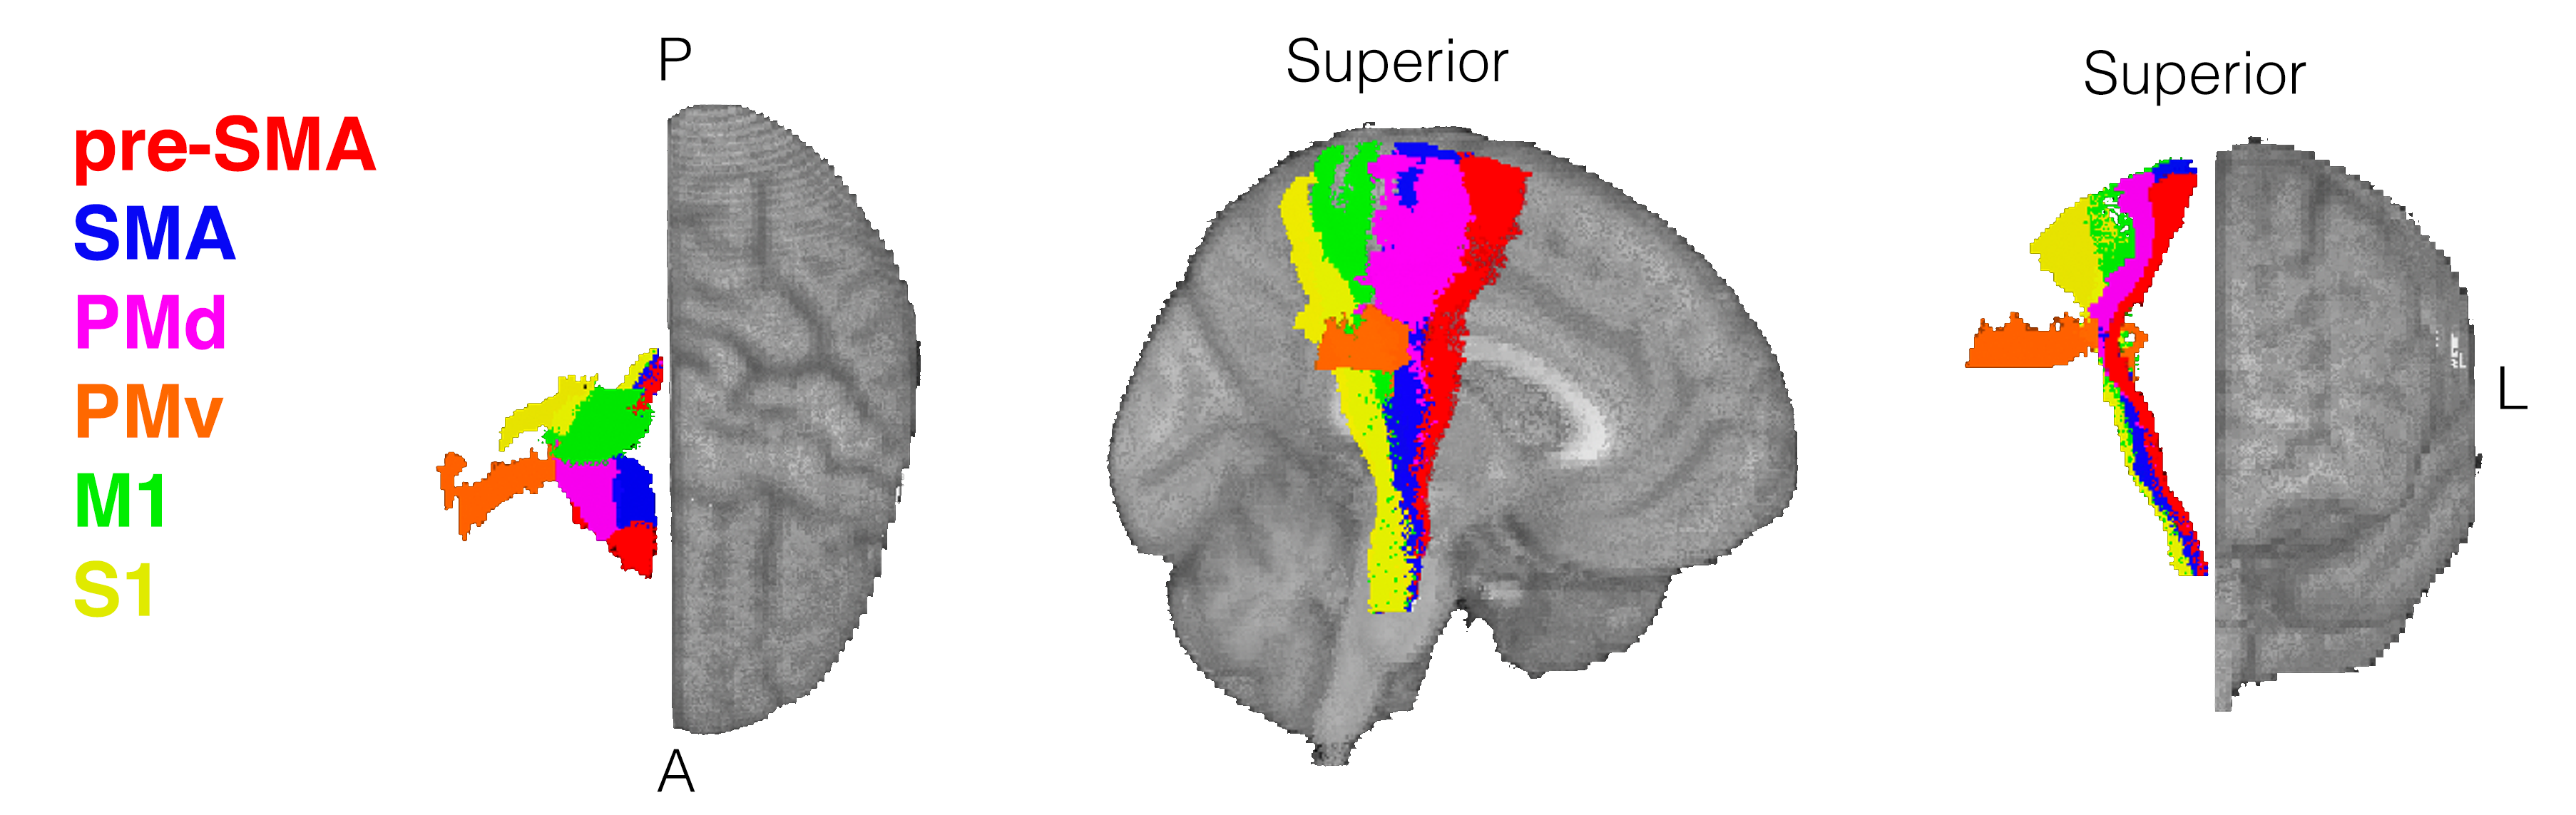
\includegraphics[width=1\linewidth]{figures/SMATT.png}
    \caption{Sensorimotor tract template atlas (SMATT), displaying only right hemisphere tracts. Includes supplementary motor area (SMA), dorsal premotor cortex (PMd), ventral premotor cortex (PMv), pre-supplementary motor area (pre-SMA), primary sensory cortex (S1),  and primary motor cortex (M1)}
    \label{smatt}
\end{figure}


Ridge regression models were used to predict chronic motor deficits from ipsilesional SMATT lesion loads (6 features) and from left/right hemisphere SMATT lesion loads (12 features). Ridge regression was used to account for multicollinearity of lesion load values between tracts (Supplementary Figure \ref{smatt_pairwise_correlations}, \ref{smatt_pairwise_correlations_bi}). Lesion load values were normalized by subtracting the mean across subjects and dividing by the l2-norm prior to model fitting. In the inner loop, the degree of regularization on regression coefficients ($\lambda$) was determined via. grid-search. The training data was fit with the selected $\lambda$ and this model was used to predict motor scores for new subjects in the test folds.


\subsubsection*{Regional change in connectivity (ChaCo) models}
Lesion masks in $1mm^3$ MNI v6 space were processed with the Network Modification Tool (NeMo Tool) v2 pipeline (\cite{Kuceyeski2013-nk}) (https://github.com/kjamison/nemo for more detailed information). Given a lesion mask, the NeMo tool produces outputs that reflect the impact of the lesion on the white matter tracts connecting brain regions. The NeMo tool identifies every white matter streamline that intersects with a lesion and determines the brain regions at the endpoints of those streamlines, whose structural connections are putatively disrupted (Figure \ref{nemo}). The NeMo tool uses a reference structural connectome dataset of 420 unrelated subjects from the Human Connectome Project (HCP) Young Adult database. Structural connectivity for HCP subjects was obtained using deterministic tractography (SD stream) with dynamic seeding, with additional SIFT2 weighting for each of 5 million streamlines (\cite{Smith2015-eb}). Regional change in connectivity (ChaCo) scores, or the ratio of the number of disrupted streamlines divided by the total number of streamlines for each region, were calculated for all grey matter regions. Regional ChaCo scores from two different altases were compared: the 86-region Desikan-Killiany Atlas (68 cortical regions $\Plus$ 18 subcortical regions, excluding brainstem) from FreeSurfer ("fs86" for short), which contains coarse anatomically parcellated regions (\cite{Desikan2006-vf,Fischl2002-lb}), and the 268-region Shen atlas ("shen268" for short), which contains more fine-grained functionally parcellated cortical and subcortical regions (\cite{Shen2013-zn}).

\begin{figure}[ht]
  \centering
  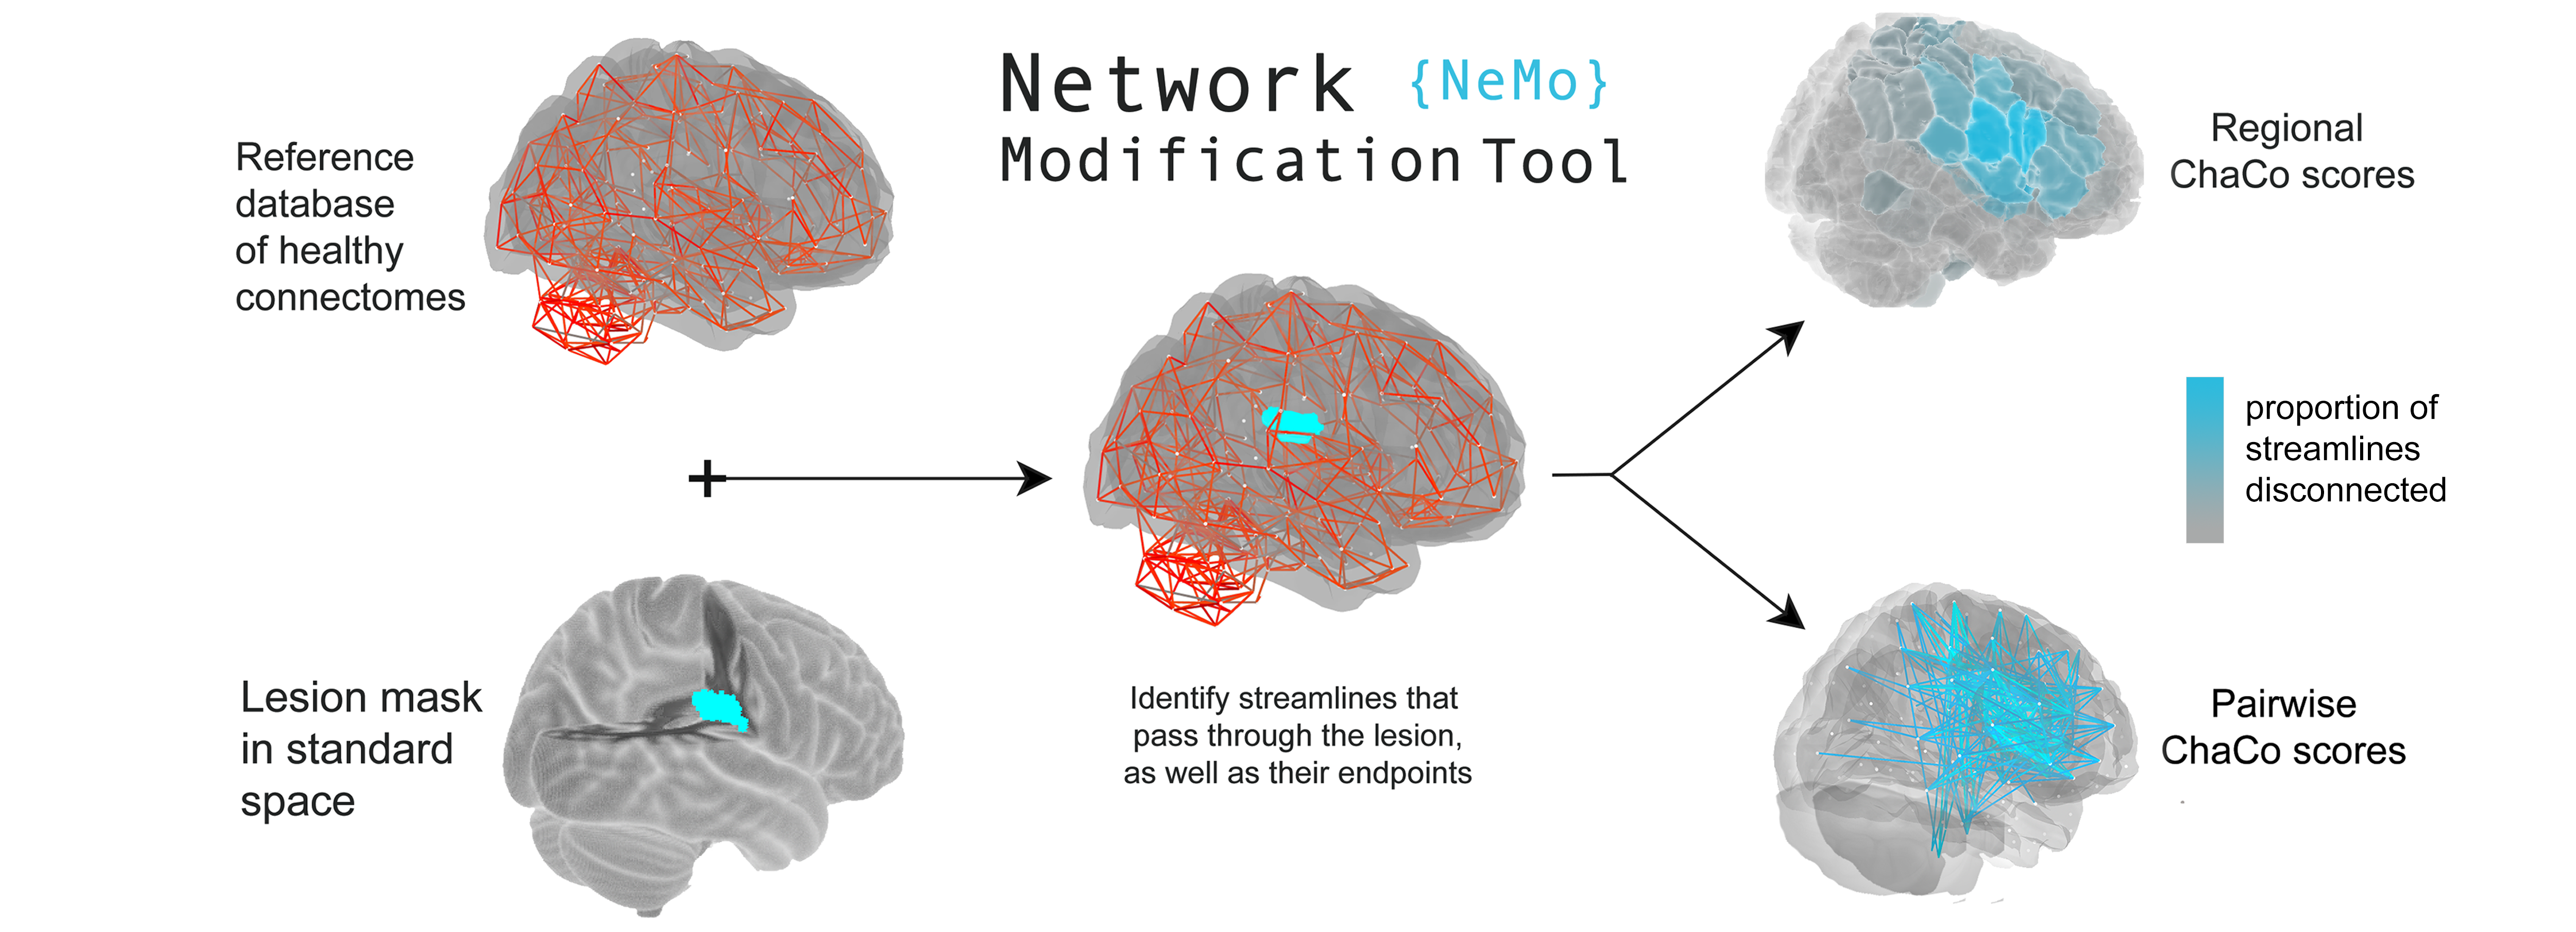
\includegraphics[width=1\linewidth]{figures/NeMo.png}
  \caption{Overview of the Network Modification tool. Binary lesion masks in MNI space representing the presence of a stroke lesion (turquoise) in a given voxel are provided by the user. Each lesion mask is embedded into 420 unrelated healthy structural connectomes (separately for each healthy subject) and the regional or pairwise change in connectivity (ChaCo) scores are calculated and averaged across healthy subjects (parcellation shown here is the Shen 268-region atlas). }
  \label{nemo}
\end{figure}

Two flavors of models using ChaCo scores were assessed. First, ridge regression models were assessed, as described above, with whole-brain regional ChaCo scores as inputs (86 features for the fs86 atlas, 268 features for the shen268 atlas). Second, a filter-based feature selection step was added to ridge regression models to obtain a subset of features that were the most useful for prediction (\cite{Hall1999-qr, Pudjihartono2022-zg}). We mixed hyperparameter tuning and feature selection in the same step, considering the feature set as a hyperparameter itself. Features were ranked by their their association with the outcome variable (p-value from univariate correlation). In the inner loop, both the amount of regularization on regression coefficients ($\lambda$) and the number of features to retain in the feature selection step ($k$) were selected via. grid search.

\subsubsection*{Visualization of feature weights}


\subsubsection*{Ensemble models}
We tested whether performance would be improved by combining several imaging biomarker metrics and/or demographic features like age, sex, and days post stroke, we used ensemble models that average predictions from different learners \cite{Hastie2001-or}. The idea of ensemble learning is to build a single prediction model by combining the strengths of a collection of simpler base models. 

We tested whether models including demographic information (age, sex, and days post stroke) alongside lesion data will perform better than models with lesion data or demographic data alone (i.e., variance explained from lesion data and demographic data is not redundant). We also assessed whether models including both lesion load and ChaCo scores will perform better than models with lesion load or ChaCo scores alone.

Ensemble models were generated by training ChaCo-models and lesion load models separately, on the same subjects and with the same training/test/validation splits, and averaging the final predicted scores for each subject. A standard linear regression model was used to model the relationship between demographic information and motor impairment. 

\subsubsection*{Code availability}
All analysis scripts that generated the results of the present study are readily accessible and open for reuse (https://github.com/emilyolafson/lesion$\_$predictions). The script can be easily modified to predict any outcome score from ChaCo scores/lesion load data.

\section{Results}

Ridge regression models fit using ChaCo scores best predicted chronic motor scores for new subjects, with an average correlation between true and predicted scores of 0.457 ($R^2 = 0.203$) and 0.456 ($R^2 = 0.199$) for the 86-region FreeSurfer atlas and 268-region Shen atlas, respectively (Figure \ref{analysis1}, Table \ref{results_table_acutechronic}). Regions whose ChaCo scores contributed most to the predictions were symmetrical across hemispheres. With both atlases, ChaCo scores in sensorimotor regions were negatively associated with motor impairment, but ChaCo scores of non-motor regions were also associated with impairment. 



\begin{table}[h]
\centering
\caption{Styled LaTeX Table}
\label{table:5}
\begin{tabular}{rrrrr}
\toprule
 &  & \multicolumn{2}{c}{Median performance} \\
 &  & Corr. (Std. dev.) & $R^2$ (Std. dev.) \\
\midrule
\multirow[t]{7}{*}{none} & M1 CST-LL & 0.394 & 0.142 \\
 & Ipsi. CST-LL & 0.430 & 0.174 \\
 & L/R CST-LL & 0.446 & 0.188 \\
 & ChaCo (shen268) (feat. select.) + demog. & 0.467 & 0.210 \\
 & ChaCo (shen268) + demog. & 0.455 & 0.199 \\
 & ChaCo (fs86) (feat. select.) + demog. & 0.447 & 0.191 \\
 & ChaCo (fs86) + demog. & 0.457 & 0.201 \\
\multirow[t]{7}{*}{demog} & M1 CST-LL+ demog. & 0.424 & 0.173 \\
 & Ipsi. CST-LL+ demog. & 0.457 & 0.199 \\
 & L/R CST-LL+ demog. & 0.462 & 0.203 \\
 & ChaCo (shen268) (feat. select.) + demog. & 0.481 & 0.215 \\
 & ChaCo (shen268) + demog. & 0.468 & 0.204 \\
 & ChaCo (fs86) (feat. select.) + demog. & 0.465 & 0.201 \\
 & ChaCo (fs86) + demog. & 0.471 & 0.203 \\
\multirow[t]{6}{*}{chaco ll} & M1 CST-LL+ ChaCo (shen268) (feat. select.) & 0.469 & 0.217 \\
 & M1 CST-LL+ ChaCo (shen268) & 0.463 & 0.211 \\
 & Ipsi. CST-LL+ ChaCo (shen268) (feat. select.) & 0.485 & 0.233 \\
 & Ipsi. CST-LL+ ChaCo (shen268) & 0.481 & 0.228 \\
 & L/R CST-LL+ ChaCo (shen268) (feat. select.) & 0.486 & 0.232 \\
 & L/R CST-LL+ ChaCo (shen268) & 0.481 & 0.228 \\
\bottomrule
\end{tabular}
\end{table}

In the interest of sharing the effects of different model parameters on prediction accuracy, we present the results of several alternative models in the supplementary materials. Although the models presented in the main paper are the strongest of all models tested, there are slight differences in the relative strengths of the alternative models. To briefly summarize: 1) in models trained only using chronic stroke subjects, ChaCo models perform approximately well as SMATT lesion load models, 2) models trained with only subjects who have Fugl-Meyer scores, and 3) models in which an additional feature selection step was employed to reduce the dimensionality of ChaCo data reduces the prediction accuracy of ChaCo models, such that SMATT lesion load models are the strongest. A brief discussion of the results of these alternative models can be found in the supplementary materials.



\begin{table}[h]
\centering
\caption{Styled LaTeX Table}
\label{table:5}
\begin{tabular}{lrrrr}
\toprule
 &  & \multicolumn{2}{c}{Median performance} \\
Ensemble type & Model name & Corr. (Std. dev.) & $R^2$ (Std. dev.) \\
\midrule
\multirow[t]{6}{*}{None} & M1 CST LL & 0.394 (0.004) & 0.142 (0.004) \\
 & Ipsi. SMATT LL & 0.430 (0.004) & 0.174 (0.004) \\
 & L/R SMATT LL & 0.446 (0.006) & 0.188 (0.006) \\
 & sLNM LL & 0.427 (0.007) & 0.165 (0.007) \\
 & ChaCo (shen268) & 0.456 (0.012) & 0.199 (0.014) \\
 & ChaCo (fs86) & 0.457 (0.008) & 0.203 (0.009) \\
\multirow[t]{6}{*}{Model plus } & M1 CST LL $\Plus$ demog. & 0.424 (0.005) & 0.173 (0.004) \\
plus demographics & Ipsi. SMATT LL $\Plus$ demog. & 0.457 (0.006) & 0.199 (0.004) \\
 & L/R SMATT LL $\Plus$ demog. & 0.462 (0.007) & 0.203 (0.004) \\
 & sLNM LL $\Plus$ demog. & 0.452 (0.006) & 0.191 (0.004) \\
 & ChaCo (shen268) $\Plus$ demog. & 0.468 (0.009) & 0.204 (0.007) \\
 & ChaCo (fs86) $\Plus$ demog. & 0.471 (0.007) & 0.203 (0.005) \\
\multirow[t]{8}{*}{Lesion load } & M1 CST LL $\Plus$ ChaCo (fs86) & 0.448 (0.005) & 0.199 (0.005) \\
 plus ChaCo & Ipsi. SMATT LL $\Plus$ ChaCo (fs86) & 0.462 (0.006) & 0.212 (0.006) \\
 & L/R SMATT LL $\Plus$ ChaCo (fs86) & 0.469 (0.005) & 0.219 (0.005) \\
 & sLNM LL $\Plus$ ChaCo (fs86) & 0.467 (0.006) & 0.214 (0.007) \\
 & M1 CST LL $\Plus$ ChaCo (shen268) & 0.466 (0.005) & 0.216 (0.004) \\
 & Ipsi. SMATT LL $\Plus$ ChaCo (shen268) & 0.478 (0.006) & 0.226 (0.006) \\
 & L/R SMATT LL $\Plus$ ChaCo (shen268) & 0.482 (0.006) & 0.230 (0.006) \\
 & sLNM LL $\Plus$ ChaCo (shen268) & 0.470 (0.008) & 0.218 (0.007) \\
\multirow[t]{8}{*}{Lesion load} & M1 CST LL $\Plus$ ChaCo  (fs86) $\Plus$ demog. & 0.473 (0.006) & 0.212 (0.005) \\
 plus ChaCo & Ipsi. SMATT LL $\Plus$ ChaCo  (fs86) $\Plus$ demog. & 0.489 (0.006) & 0.228 (0.005) \\
 plus demographics & L/R SMATT LL $\Plus$ ChaCo  (fs86) $\Plus$ demog. & 0.491 (0.006) & 0.228 (0.005) \\
 & sLNM LL $\Plus$ ChaCo  (fs86) $\Plus$ demog. & 0.485 (0.006) & 0.221 (0.005) \\
 & M1 CST LL $\Plus$ ChaCo  (shen268) $\Plus$ demog. & 0.483 (0.006) & 0.222 (0.005) \\
 & Ipsi. SMATT LL $\Plus$ ChaCo  (shen268) $\Plus$ demog. & 0.500 (0.007) & 0.237 (0.006) \\
 & L/R SMATT LL $\Plus$ ChaCo  (shen268) $\Plus$ demog. & 0.499 (0.007) & 0.237 (0.006) \\
 & sLNM LL $\Plus$ ChaCo  (shen268) $\Plus$ demog. & 0.487 (0.006) & 0.224 (0.005) \\

 \arrayrulecolor{black}\bottomrule
\end{tabular}
\caption{Test performance of all models evaluated, displaying median $R^2$ and median correlation of average hold-out performances (i.e. average across 5 outer folds) across 100 permutations. The first 5 rows contain results from models using lesion information only. The second 5 rows contain results from ensemble models that average predictions from lesion information and demographcis (age, sex, days post stroke). The final 6 rows contain results from ensemble models averaging predictions between two types of lesion information (lesion load predictions and ChaCo score predictions), with the final 3 rows showing results from ensemble models using lesion load, ChaCo scores, and demographics. Demog. = demographics, Ipsi. = Ipsilesional, SMATT LL = sensorimotor tract template lesion load, L/R SMATT LL = left and right sensorimotor tract template lesion load, M1 CST LL = M1 corticospinal tract lesion load, ChaCo = Change in Connectivity, fs86 = FreeSurfer 86-region atlas}
\label{results_table_acutechronic}

\end{table}



\begin{figure}[htp]
\centering
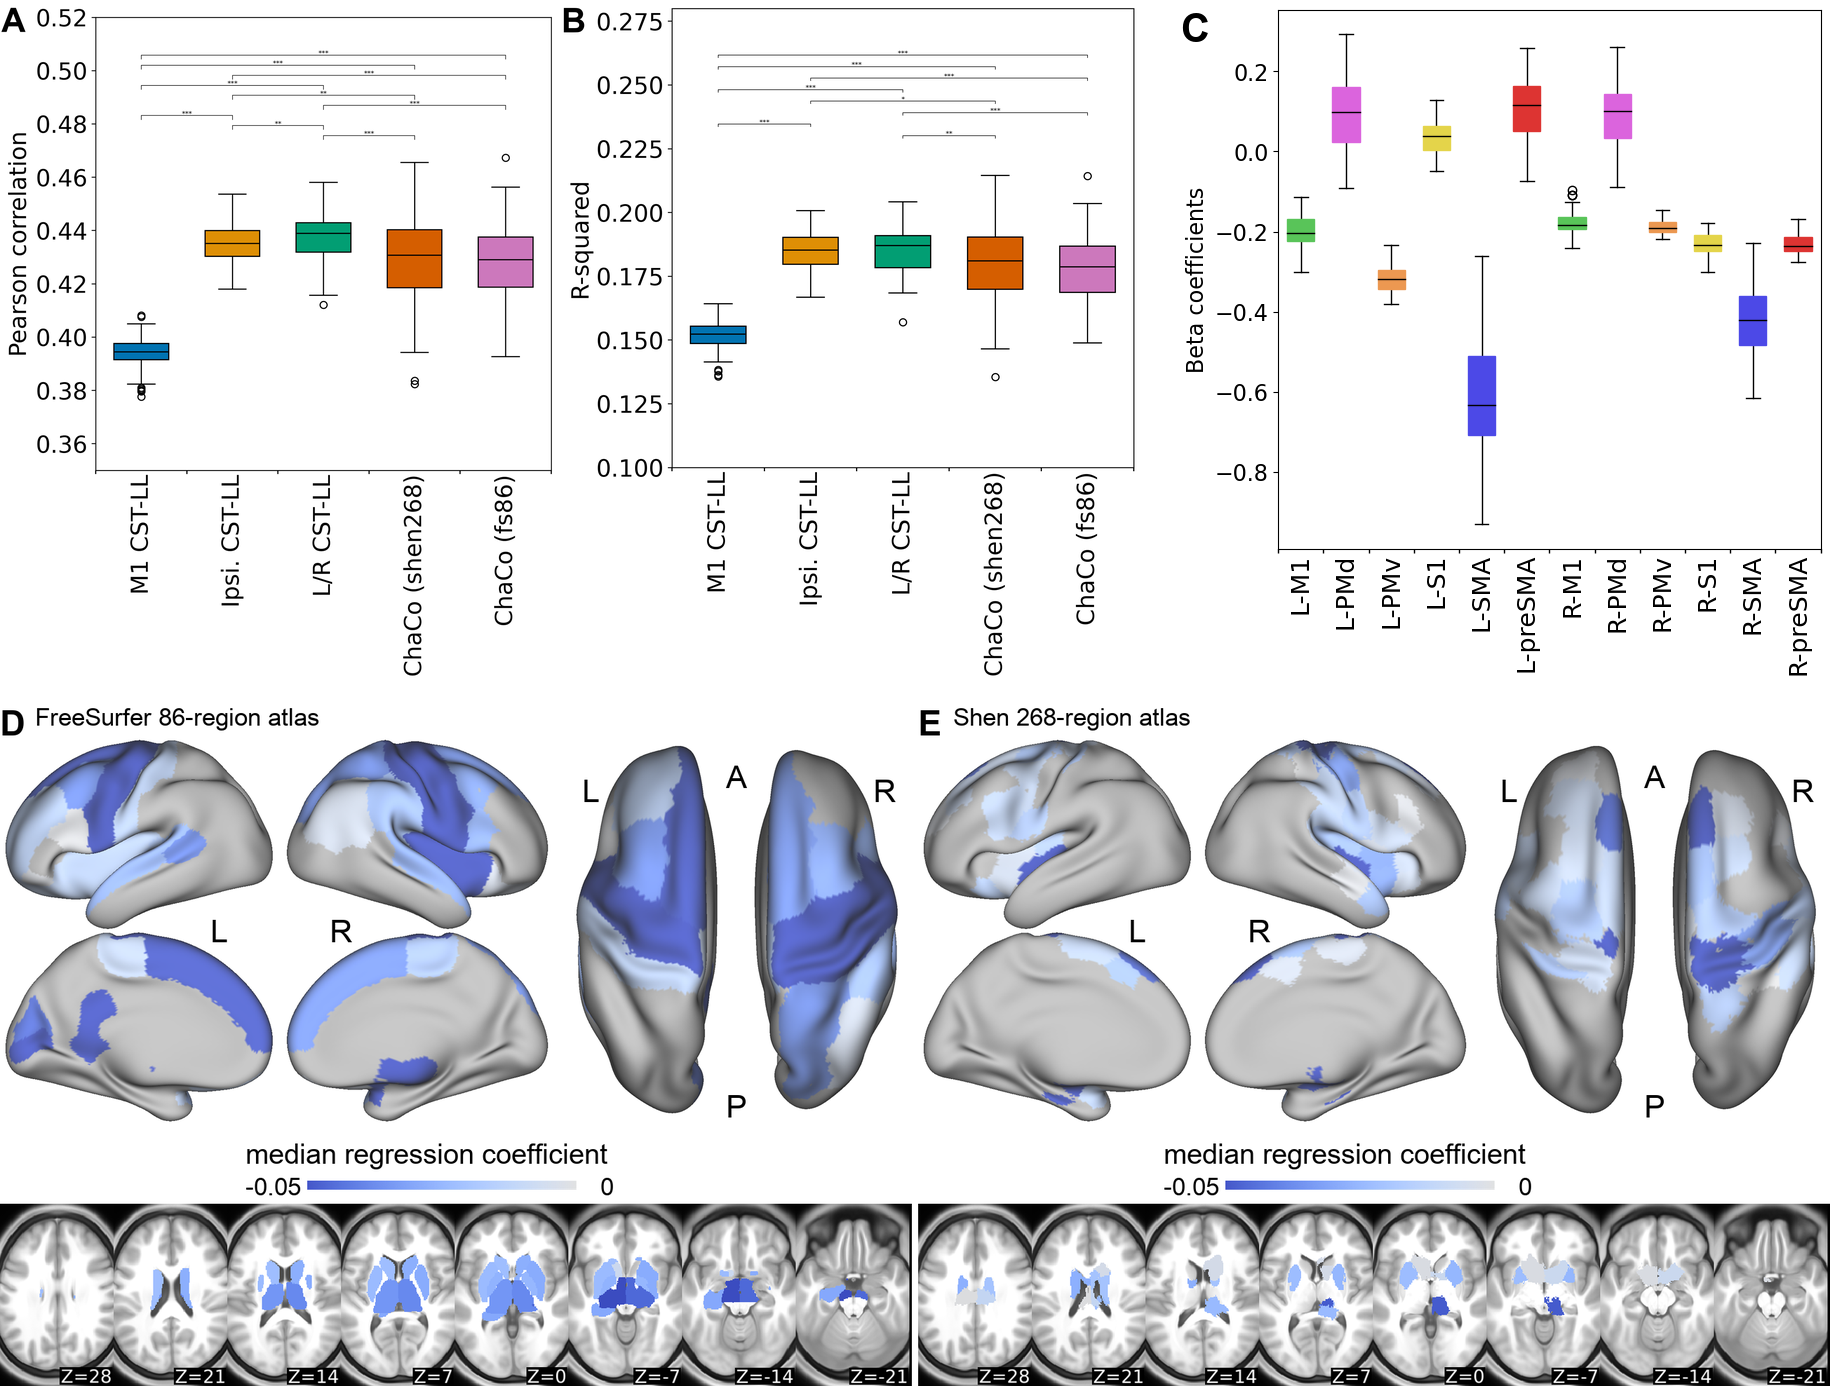
\includegraphics[width=1\linewidth]{figures/Analysis1.png}
\caption{Regression coefficients and model performance using standard KFold cross-validation (train/test splits shuffled). \textbf{A.} and \textbf{B.} display model performance (mean Pearson correlation/$R^2$ across 5 outer folds for 100 permutations of the data). Boxplots are colored abritrarily for clarify, where the box extends from the lower to upper quartile values of the data, with a line at the median. Whiskers represent the range of the data from [Q1-1.5*IQR, Q3+1.5*IQR].
Average feature weights for regions that were selected in at least half of the models (i.e., were included in the model in at least 250/500 outer folds). \textbf{C.} Sensorimotor area tract template feature importance for analysis 1. Includes primary motor cortex (M1), dorsal premotor cortex (PMd), ventral premotor cortex (PMv), supplementary motor area (SMA), pre-supplementary motor area (pre-SMA), primary sensory cortex (S1).}
\label{analysis1}
\end{figure}

\begin{figure}[htp]
\centering
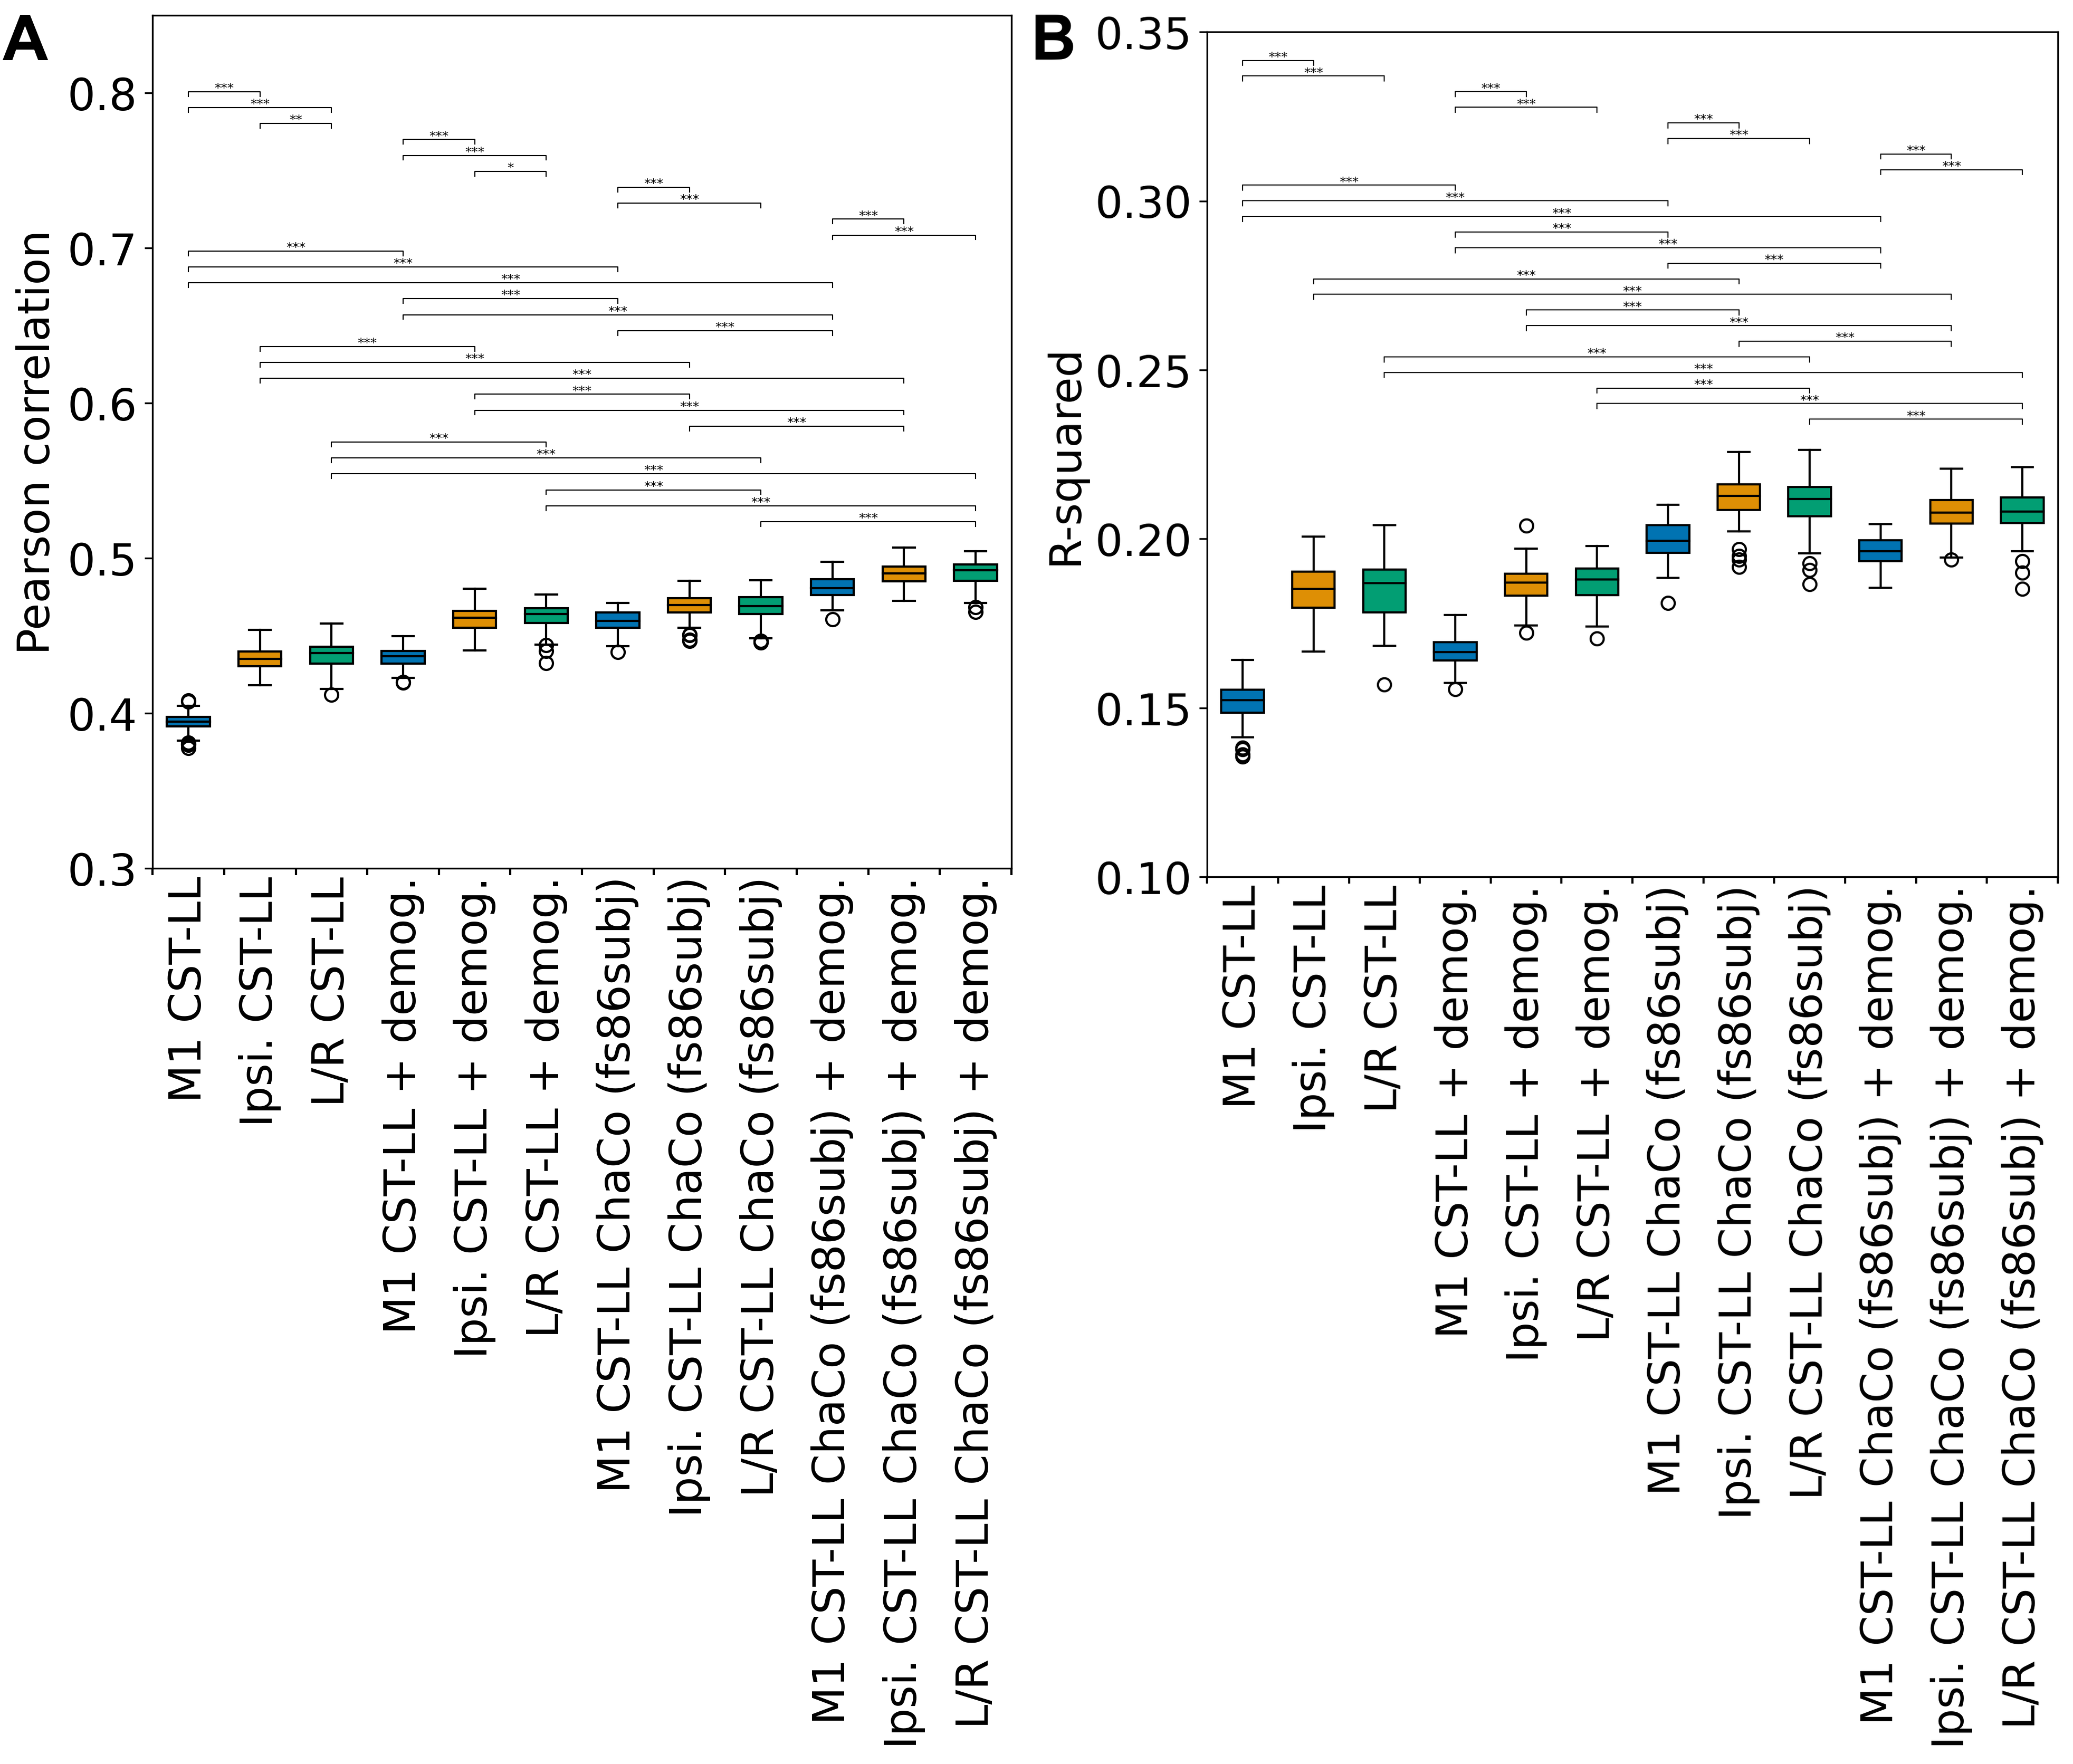
\includegraphics[width=1\linewidth]{figures/Analysis2.png}
\caption{Ensemble model results. coefficients and model performance using Group KFold cross-validation (test/validate on independent imaging site). \textbf{A.} and \textbf{B.} display regression coefficients for regional ChaCo scores (FreeSurfer 86-region atlas, and Shen268-region atlas, respectively). Average feature weights for regions that were selected in at least half of the models (i.e., were included in the model in at least 250/500 outer folds). \textbf{C.} Sensorimotor area tract template feature importance for analysis 2. Includes primary motor cortex (M1), dorsal premotor cortex (PMd), ventral premotor cortex (PMv), supplementary motor area (SMA), pre-supplementary motor area (pre-SMA), primary sensory cortex (S1).}
\label{nemotool}
\end{figure}



\section{Discussion}

\clearpage



\printbibliography
\section*{Supplementary Results}

\beginsupplement
\begin{figure}[ht]
\centering
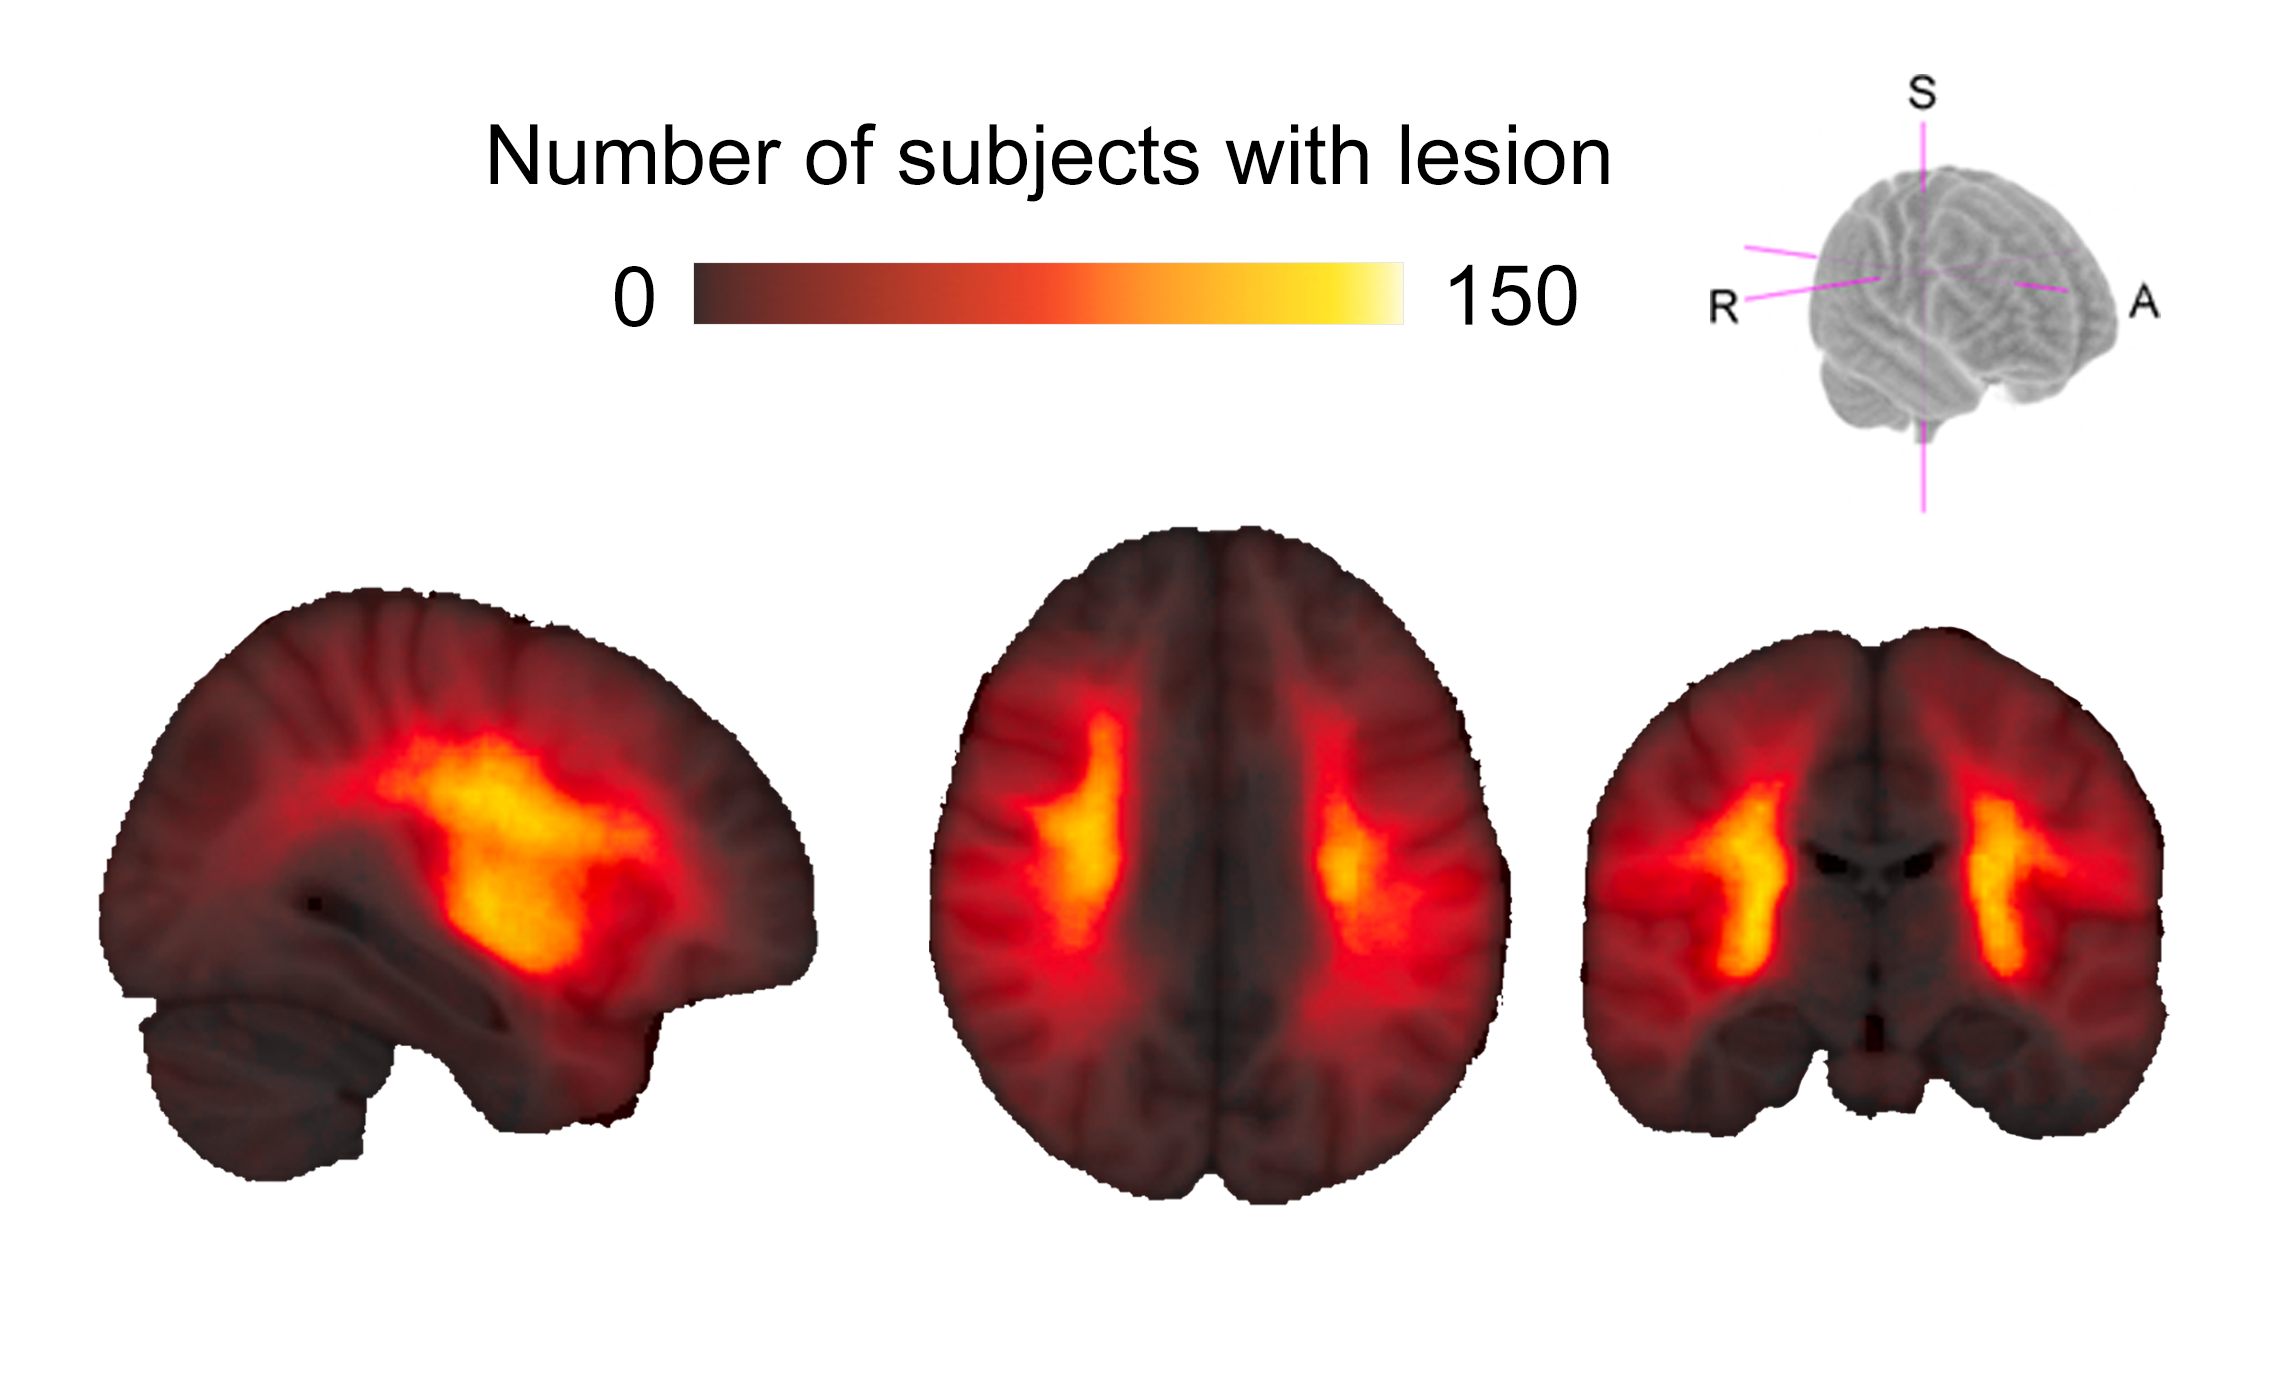
\includegraphics[width=0.8\linewidth]{figures/distribution_lesions.png}
\caption{Distribution of lesions in ENIGMA cohort.}
\label{lesiondist}
\end{figure}

\begin{figure}
\begin{subfigure}{0.5\textwidth}
  \centering
  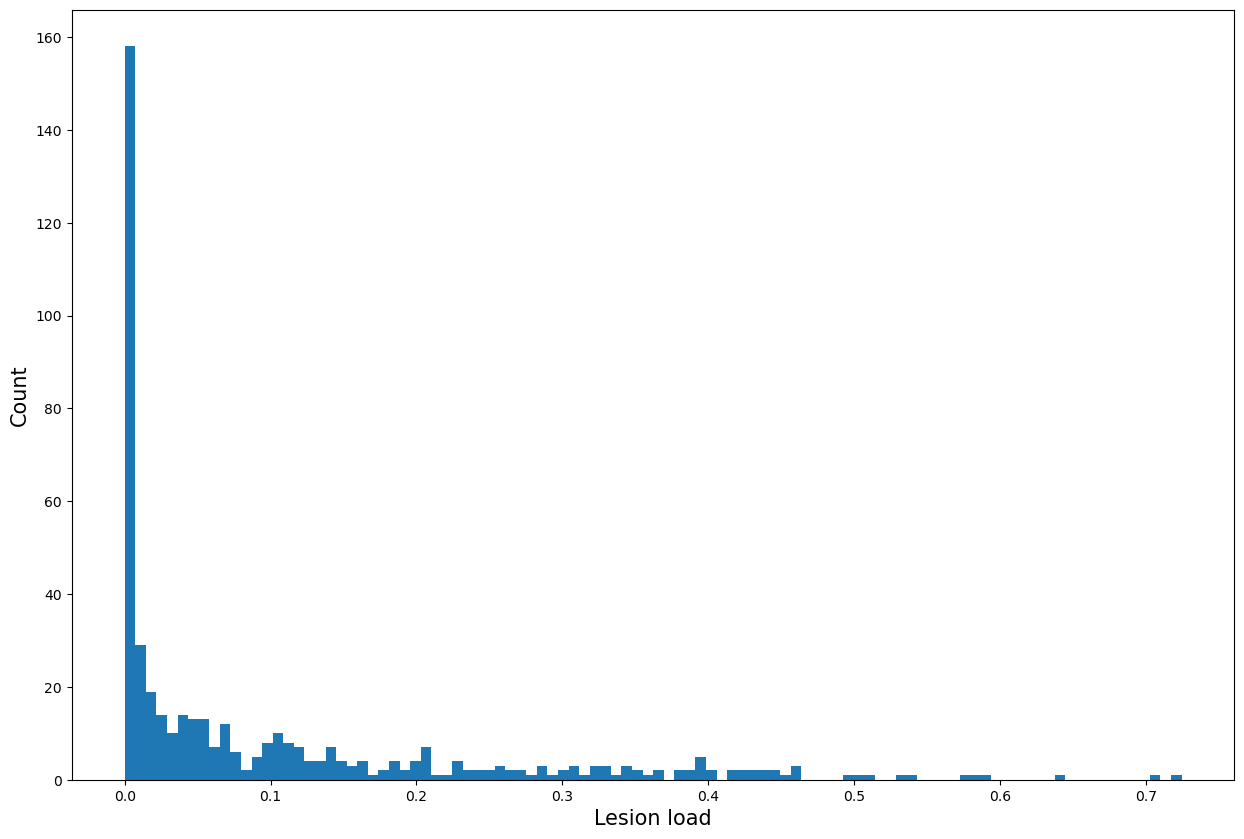
\includegraphics[width=1\linewidth]{figures/m1_lesionload.png}
  \caption{M1-CST lesion load distribution.}
  \label{fig:sfig1}
\end{subfigure}
\begin{subfigure}{0.5\textwidth}
  \centering
  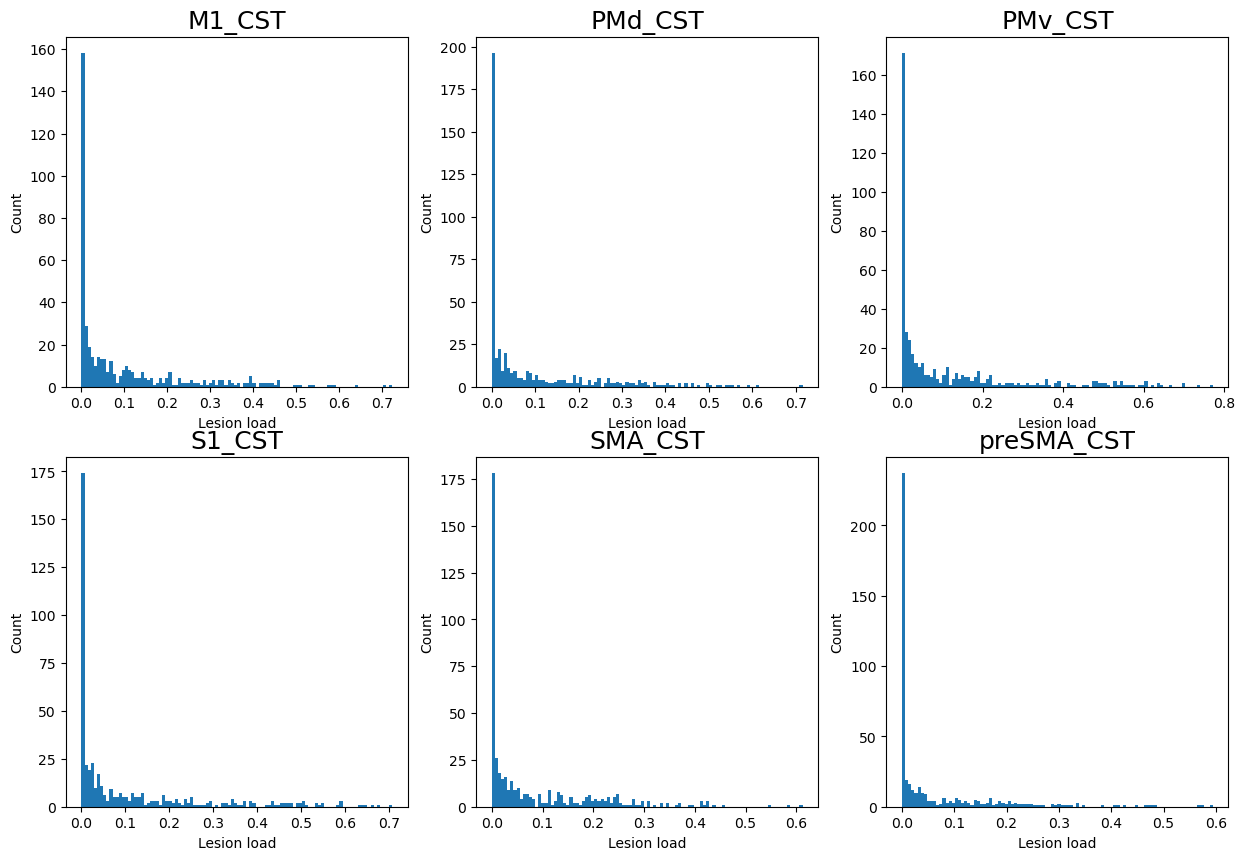
\includegraphics[width=1\linewidth]{figures/all_lesionload.png}
  \caption{Ipsilesional sensorimotor tract template (SMATT) lesion load distribution.}
  \label{fig:sfig2}
\end{subfigure}
\begin{subfigure}{1\textwidth}
  \centering
  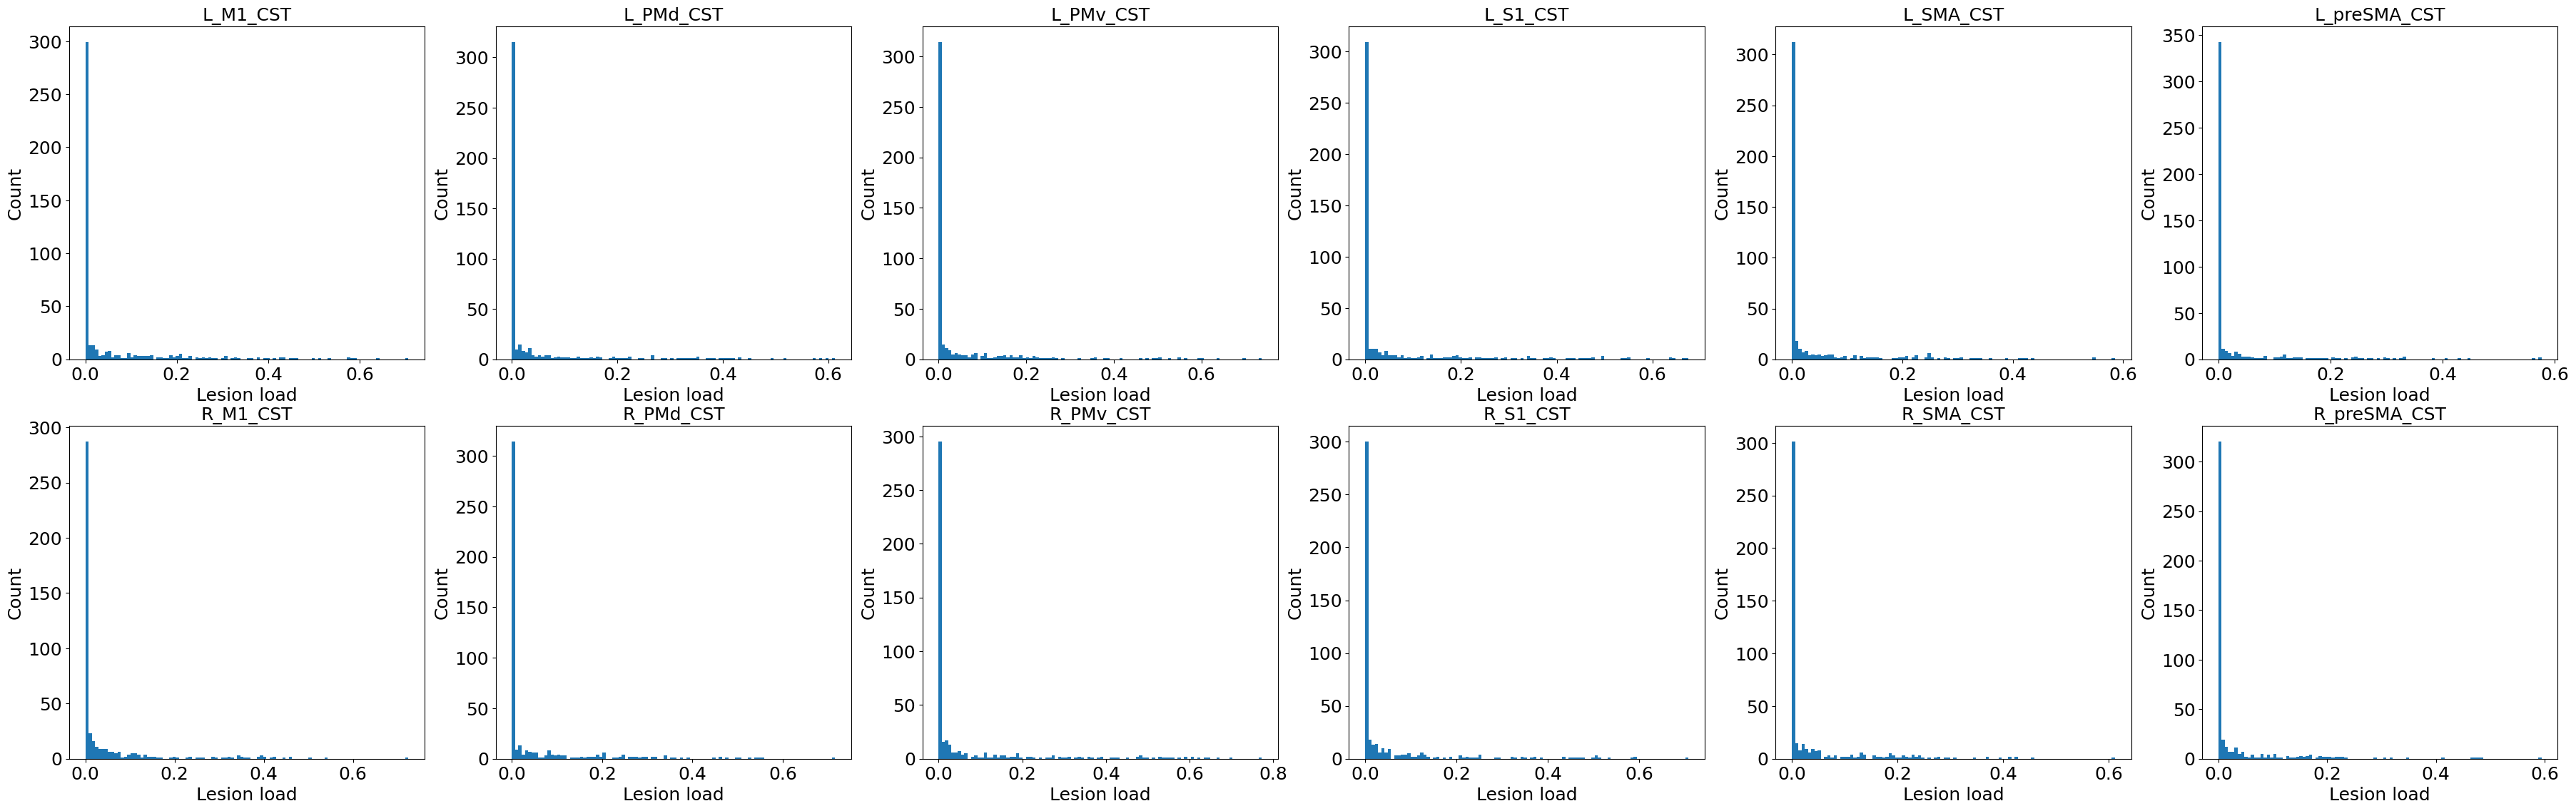
\includegraphics[width=1\linewidth]{figures/all2h_lesionload.png}
  \caption{Left and right hemisphere sensorimotor tract template (SMATT) lesion load distribution.}
  \label{fig:sfig2}
\end{subfigure}
\caption{Distribution of lesion load variables for chronic subjects.}
\label{lesion_load_dist}
\end{figure}


\begin{figure}[ht]
\centering
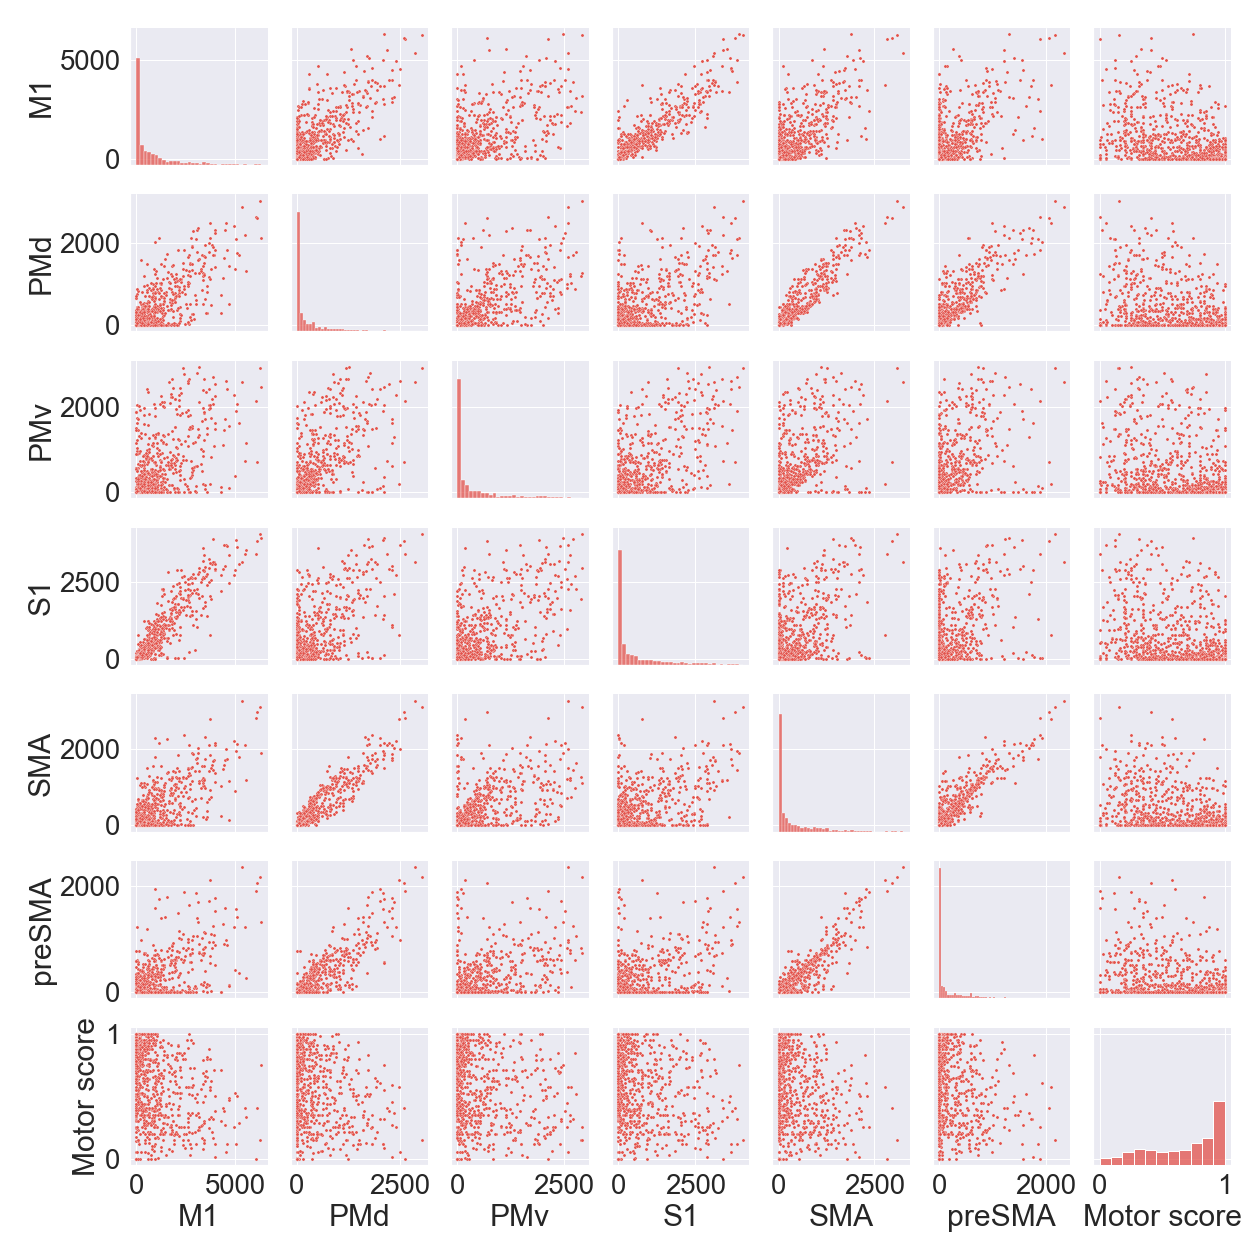
\includegraphics[width=0.8\linewidth]{figures/SMATT_scatterplts.png}
\caption{Correlations between lesion load calculated for each ipsilesional tract in the sensorimotor area tract template atlas.}
\label{smatt_pairwise_correlations}
\end{figure}

\begin{figure}[ht]
\centering
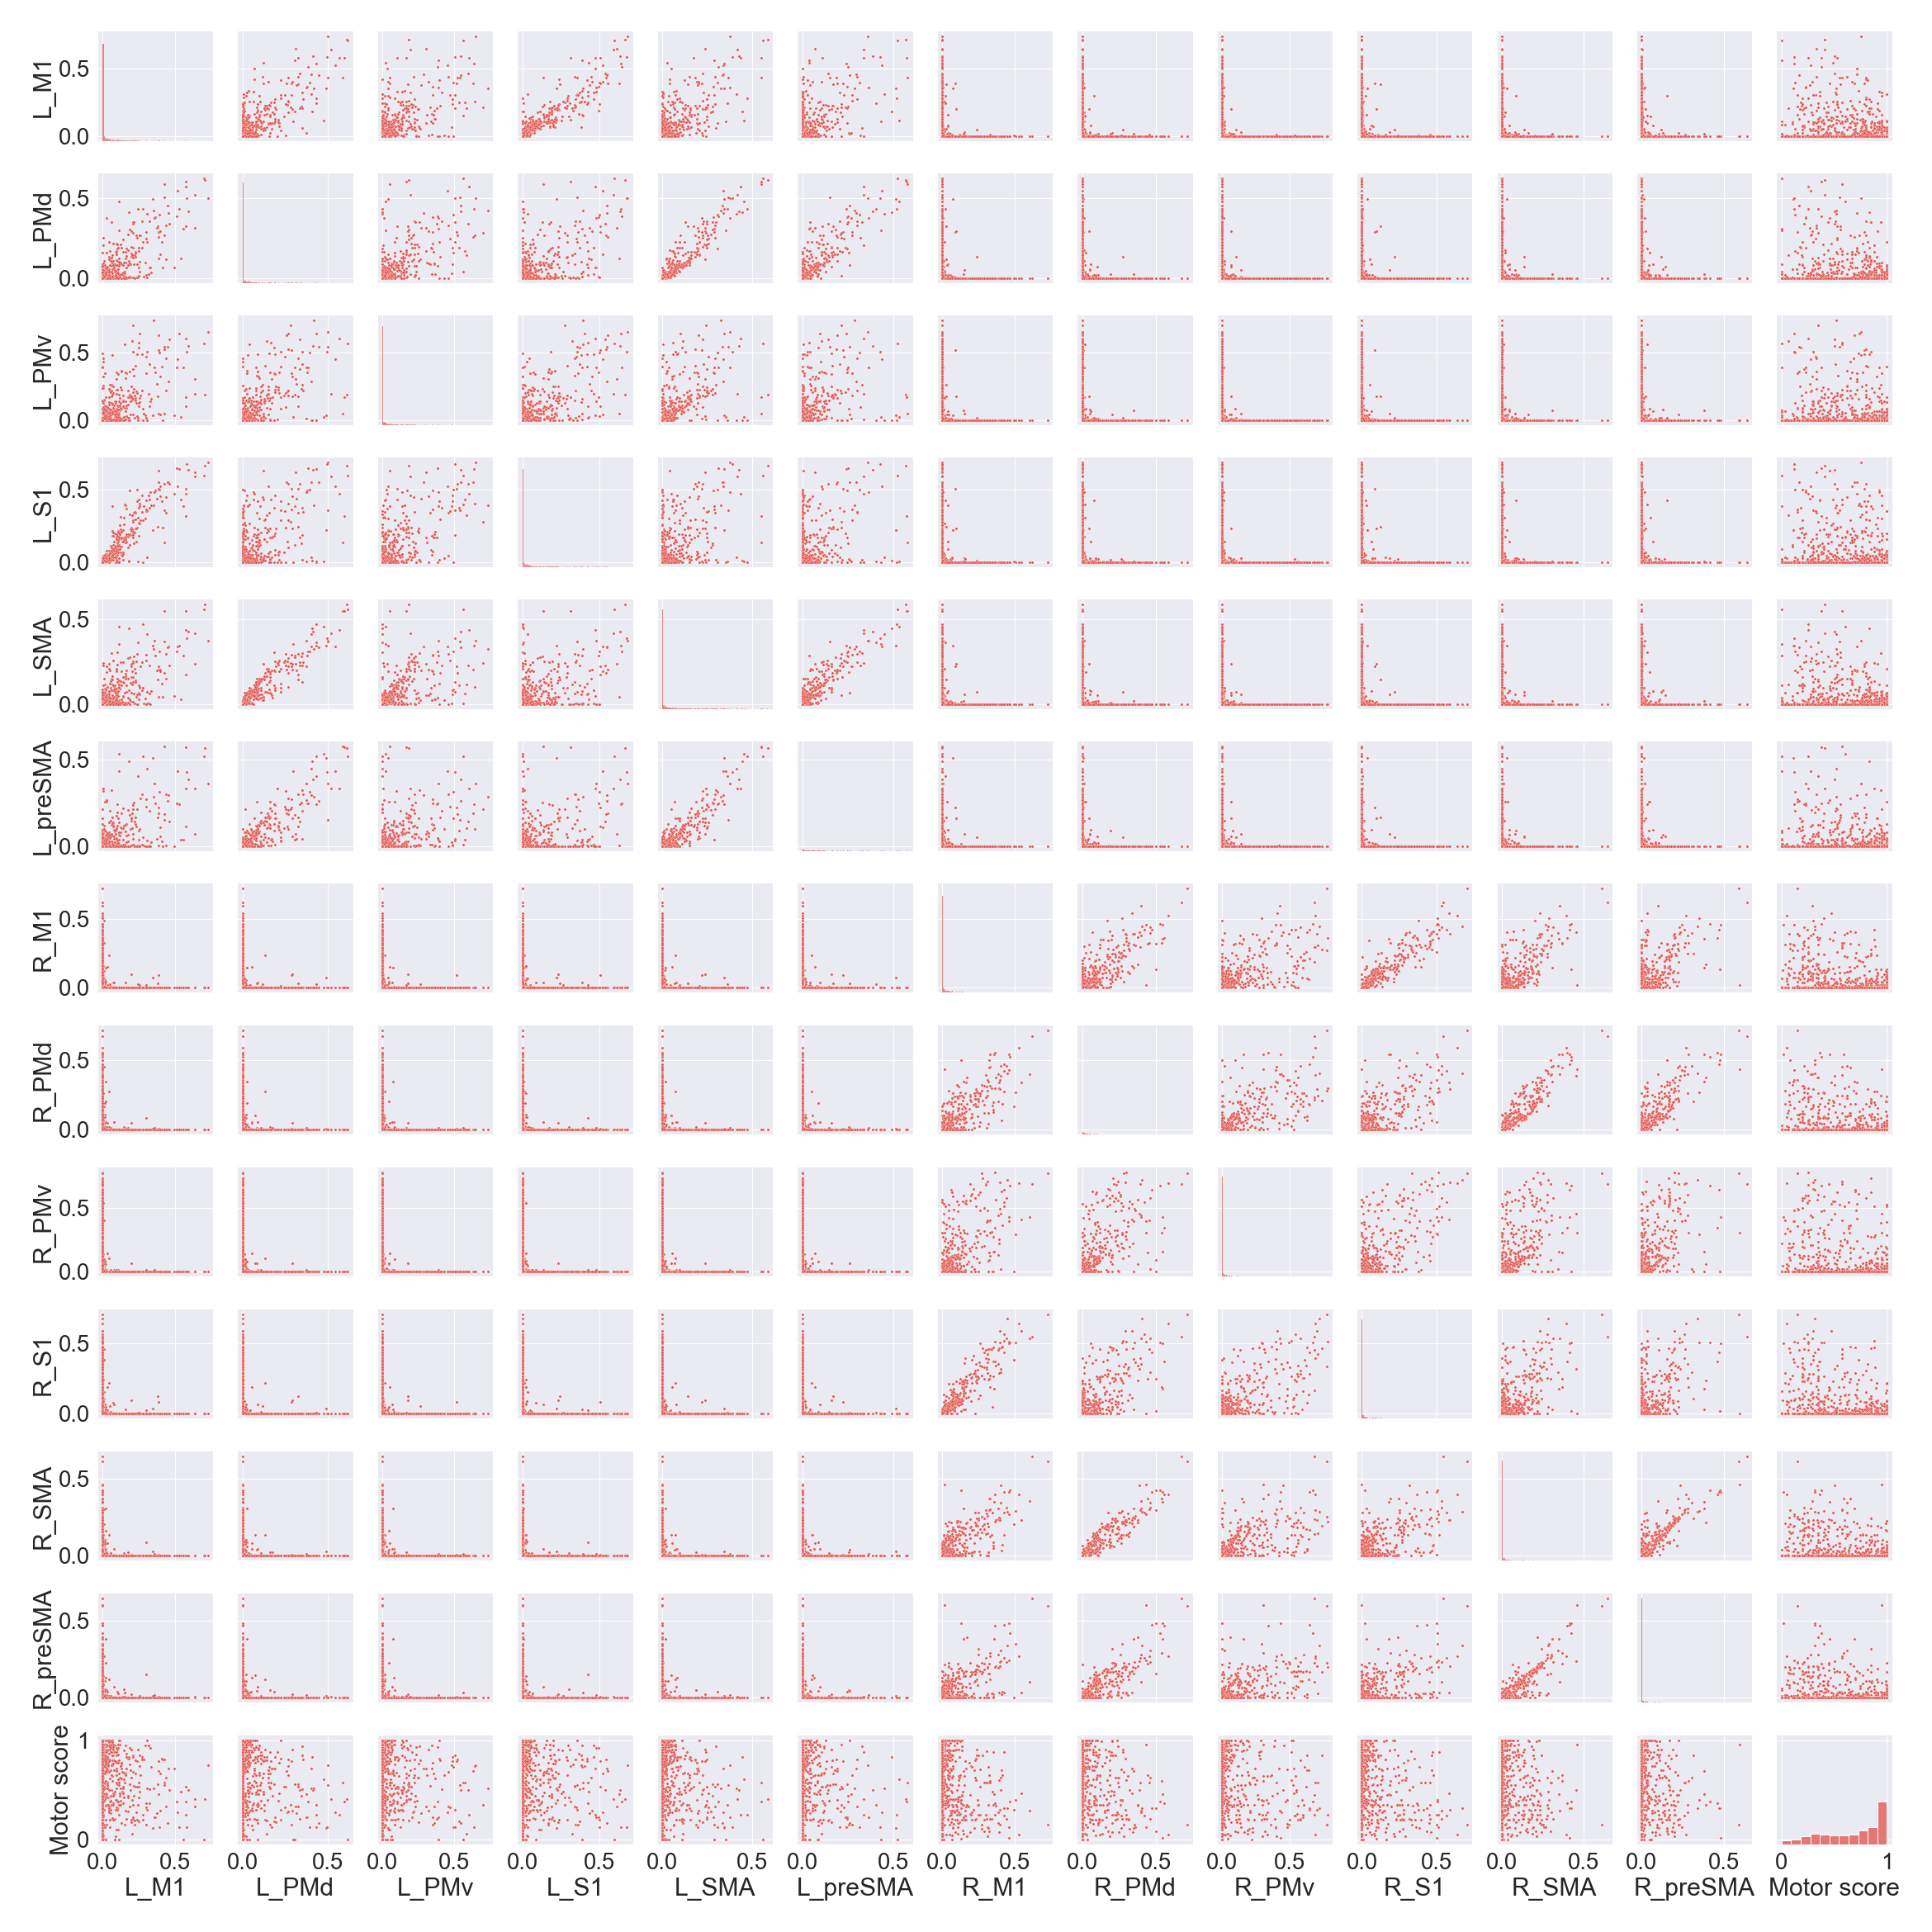
\includegraphics[width=1\linewidth]{figures/SMATT_bi_scatterplts.png}
\caption{Correlations between lesion load calculated for each left and right hemisphere tract in the sensorimotor area tract template atlas.}
\label{smatt_pairwise_correlations_bi}
\end{figure}


\end{document}